% Snowflake Data Engineering — Chapter 8 | original manuscript draft
% Author: Arman Golbidi | Editorial snapshot: 22 October 2026
% Compile: xelatex -interaction=nonstopmode -halt-on-error Snowflake_Data_Engineering_Chapter_08.tex
% Trim: 178 x 254 mm; margins inside 23 mm / outside 17 mm / top-bottom 19 mm.
% Body: 10.75 pt / 13.65 pt leading = 1.27 line-height ratio; code: 8.75 pt.
\documentclass[11pt,twoside]{article}
\usepackage[paperwidth=178mm,paperheight=254mm,inner=23mm,outer=17mm,top=19mm,bottom=19mm,headheight=5mm,headsep=4mm,footskip=9mm]{geometry}
\usepackage{fontspec}
\setmainfont{LibertinusSerif-Regular.otf}[BoldFont=LibertinusSerif-Bold.otf,ItalicFont=LibertinusSerif-Italic.otf,BoldItalicFont=LibertinusSerif-BoldItalic.otf]
\setsansfont{LibertinusSans-Regular.otf}[BoldFont=LibertinusSans-Bold.otf,ItalicFont=LibertinusSans-Italic.otf]
\setmonofont{LibertinusMono-Regular.otf}[Scale=0.91]
\usepackage[english]{babel}
\usepackage{microtype}
\usepackage{setspace}
\setstretch{1.0}
\usepackage{titlesec,enumitem,tabularx,array,booktabs,needspace,fancyhdr,lastpage}
\usepackage[most]{tcolorbox}
\usepackage{tikz}
\usetikzlibrary{arrows.meta,positioning,fit,shapes.misc,calc}
\usepackage{listings}
\usepackage{xcolor}
\usepackage{hyperref}
\usepackage{amsmath}
\hypersetup{colorlinks=true,urlcolor=steelblue,linkcolor=steelblue,pdfauthor={Arman Golbidi},pdftitle={Snowflake Data Engineering - Chapter 8: Streams, Tasks, and Dynamic Tables},pdfsubject={English technical book manuscript, eighth chapter, 178 x 254 mm}}
\definecolor{navy}{HTML}{15334A}
\definecolor{steelblue}{HTML}{17779B}
\definecolor{teal}{HTML}{12888A}
\definecolor{lightblue}{HTML}{ECF5F7}
\definecolor{papergray}{HTML}{F2F5F6}
\definecolor{inkgray}{HTML}{4A5862}
\definecolor{thinrule}{HTML}{CBD7DB}
\AtBeginDocument{\color{navy}\fontsize{10.75}{13.65}\selectfont}
\setlength{\parindent}{0pt}
\emergencystretch=2.5em
\setlength{\parskip}{3.3pt plus 0.7pt minus 0.6pt}
\setlist[itemize]{leftmargin=4mm,itemsep=1pt,topsep=2pt,parsep=0pt}
\setlist[enumerate]{leftmargin=5mm,itemsep=1pt,topsep=2pt}
\titleformat{\section}{\sffamily\bfseries\color{navy}\fontsize{14}{17}\selectfont}{}{0pt}{}
\titlespacing*{\section}{0pt}{8pt}{4pt}
\titleformat{\subsection}{\sffamily\bfseries\color{steelblue}\fontsize{10.8}{13}\selectfont}{}{0pt}{}
\titlespacing*{\subsection}{0pt}{5pt}{1pt}
\newcommand{\topic}[2]{\subsection*{#1\quad #2}}
\newcommand{\repo}[2]{\par\begingroup\fontsize{8.0}{9.6}\selectfont\sffamily\color{inkgray}\textbf{Project reference:} \href{#2}{#1}. \textit{Not independently executed; rights review pending.}\par\endgroup}
\newtcolorbox{insight}[1][]{enhanced,breakable,colback=lightblue,colframe=thinrule,boxrule=.45pt,arc=1.3mm,left=2.8mm,right=2.8mm,top=1.8mm,bottom=1.8mm,before skip=5pt,after skip=5pt,#1}
\newtcolorbox{whitebox}[1][]{enhanced,breakable,colback=papergray,colframe=thinrule,boxrule=.35pt,arc=1mm,left=2.6mm,right=2.6mm,top=1.5mm,bottom=1.5mm,before skip=4pt,after skip=5pt,#1}
\lstdefinestyle{chaptercode}{basicstyle=\ttfamily\fontsize{8.75}{10.7}\selectfont,backgroundcolor=\color{papergray},frame=single,framerule=.35pt,rulecolor=\color{thinrule},breaklines=true,columns=fullflexible,keepspaces=true,showstringspaces=false,aboveskip=5pt,belowskip=5pt,xleftmargin=2mm,xrightmargin=1mm,framexleftmargin=2mm,framexrightmargin=1mm}
\lstset{style=chaptercode}
\pagestyle{fancy}
\fancyhf{}
\fancyhead[LE]{\sffamily\fontsize{7.6}{9}\selectfont\color{inkgray}\textsc{Snowflake Data Engineering}}
\fancyhead[RO]{\sffamily\fontsize{7.6}{9}\selectfont\color{inkgray}\textsc{08 / Incremental Pipelines}}
\fancyfoot[LE,RO]{\sffamily\bfseries\fontsize{8.2}{9}\selectfont\color{steelblue}\thepage}
\fancyfoot[LO,RE]{\sffamily\fontsize{7.6}{9}\selectfont\color{inkgray}Arman Golbidi \quad | \quad Chapter 08}
\renewcommand{\headrulewidth}{0.35pt}
\renewcommand{\footrulewidth}{0pt}
\setcounter{page}{133}
\raggedbottom

% CHAPTER 08 ONLY, pages 133--150 in the planned book
\begin{document}
% PAGE 133 — chapter opening
{\sffamily\bfseries\fontsize{9}{11}\selectfont\color{steelblue} CHAPTER 08 \hfill DATA ENGINEERING / INCREMENTAL SYSTEMS}\par\vspace{3mm}
{\sffamily\bfseries\fontsize{21.2}{24.5}\selectfont\color{navy} Streams, Tasks, and\\Dynamic Tables}\par\vspace{2mm}
{\sffamily\fontsize{11.1}{14}\selectfont\color{steelblue} Make changed data useful without rebuilding the world}\par\vspace{4mm}
\begin{insight}\textbf{A correction is not another megawatt-hour.}\par
An operator opens the Finland Energy Analytics dashboard at 10:15. Wind generation for 10:00 is shown as 12 MWh, although a corrected reading of 14 MWh arrived five minutes earlier. A naive pipeline appends both observations to a daily aggregate and displays 26 MWh. The ingestion service did its job, but the analytical result is wrong. The system needs not only rapid delivery, but an unambiguous rule for \emph{which version of a business fact is current}, together with a dependable method for maintaining that rule as changes arrive.\end{insight}
Chapter~7 established a safe bronze ingestion boundary: events carry identity, UTC interval, revisions, and records of retry and validation. This chapter consumes that boundary. We compare two styles of downstream maintenance: \emph{procedural} change consumption using Snowflake Streams and Tasks, and \emph{declarative} materialisation using Dynamic Tables. Both solve meaningful problems; neither can repair an unspecified business contract.
\begin{whitebox}\textbf{Learning outcomes}\par
After this chapter, you should be able to: (1) reason about insert, update, delete and replay semantics; (2) explain stream offsets, transactional consumption and staleness; (3) build a deterministic \texttt{MERGE} with a triggered Task; (4) specify a Dynamic Table with an intentional refresh mode and target lag; (5) compare consistency, freshness, observability, cost and recovery; and (6) reconcile two implementations on a controlled energy fixture.\end{whitebox}
\textbf{Prerequisites.} Chapters~5--7, SQL joins and window functions from Chapter~4, and a basic understanding of change data capture. The offline laboratory uses Python~3.10+ without external packages; SQL templates require an authorised Snowflake account and have \emph{not} been executed there.
\begin{center}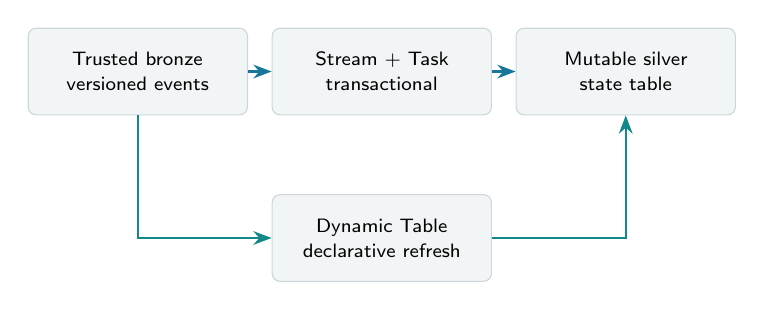
\begin{tikzpicture}[>=Stealth,every node/.style={font=\sffamily\fontsize{7.4}{9}\selectfont}, n/.style={draw=thinrule,rounded corners=1mm,fill=papergray,align=center,text width=25.5mm,minimum height=11mm}]
\node[n](a){Trusted bronze\\versioned events};\node[n,right=3mm of a](b){Stream + Task\\transactional};\node[n,right=3mm of b](c){Mutable silver\\state table};\node[n,below=10mm of b](d){Dynamic Table\\declarative refresh};
\draw[->,thick,steelblue](a)--(b);\draw[->,thick,steelblue](b)--(c);\draw[->,thick,teal](a.south)|-(d.west);\draw[->,thick,teal](d.east)-|(c.south);
\end{tikzpicture}\\{\fontsize{8}{9.5}\selectfont\color{inkgray}Figure 8.1. Alternative paths to a comparable current-state view; not one pipeline requiring both.}\end{center}
\newpage
%PAGE
% PAGE 134 — 8.1.1
\section*{8.1\quad Change data capture and incremental updates}
\topic{8.1.1}{Change data capture as an information contract}
Change data capture (CDC) describes changes to a source dataset rather than transmitting a complete current snapshot after every alteration. In a database log, CDC may identify committed INSERT, UPDATE and DELETE operations. In an event feed, what looks like CDC can instead be a collection of immutable \emph{revision events}: the original measurement remains in the log and a later event states a better value. These two encodings are not automatically interchangeable. Snowflake Streams expose change tracking over a supported source object; they do \emph{not} magically supply business meaning when an upstream event is a correction rather than a SQL UPDATE.

For the energy example, define business key \(K=(provider,technology,interval\_utc)\). The provider identifies the source authority, technology identifies the energy category and the interval represents a UTC measurement grain, not a wall-clock label in Europe/Helsinki. A new event contains \texttt{revision}, \texttt{event\_id}, \texttt{operation} and its measurement. The business contract is \emph{highest approved revision wins}. This is different from last record received wins: delayed networks may deliver a newer revision first and an obsolete correction later.
\begin{center}\renewcommand{\arraystretch}{1.12}\begin{tabularx}{\linewidth}{@{}p{18mm}p{21mm}X@{}}\toprule
\textbf{Time}&\textbf{Message}&\textbf{Required result}\\\midrule
10:00&Wind r1: 12&Current wind = 12 MWh\\
10:05&Wind r2: 14&Replace; current wind = 14 MWh\\
10:06&Wind r1: 12&Ignore obsolete replay; still 14 MWh\\
10:07&Wind r2: 14&Duplicate: one effective version\\\bottomrule
\end{tabularx}\\{\fontsize{8}{9.5}\selectfont\color{inkgray}Table 8.1. Arrival order and revision order are not equivalent.}\end{center}
A CDC feed should publish a documented rule for transaction boundaries, primary keys, deletes and retention. Without it, two consumers can independently produce incompatible totals while both pipelines appear operational. The rule for energy is especially important: summing raw received versions creates double-counting, so the silver table must resolve state before an analytical aggregate is calculated.
\begin{whitebox}\textbf{Decision test}\par
Is the source a database table emitting row-level mutations, an append-only audit log, or a revisioned measurement API? Identify the difference first. If you cannot state what a DELETE means for a business key and whether the next lower revision may reappear, do not choose the ingestion operator yet.\end{whitebox}
\repo{P081: PostgreSQL CDC to Snowflake reference}{https://github.com/Snowflake-Labs/sfguide-intro-to-cdc-using-snowflake-postgres-connector-dynamic-tables}
\textbf{Check.} Which key prevents the 10:00 wind reading from being counted twice, and why is \texttt{received\_at} an inadequate sole conflict-resolution field?
\newpage
%PAGE
% PAGE 135 — 8.1.2
\topic{8.1.2}{Inserts, updates, deletes, and tombstones}
In a state table, INSERT creates a previously unknown row, UPDATE changes attributes of an existing row, and DELETE removes it from that table's current state. Yet these physical operations do not necessarily preserve an audit trail. The bronze event log should normally retain the original delivery for traceability, within an approved retention and privacy policy. Silver can store one current state per key, with a flag or operation marker indicating that the latest approved revision is a deletion.

A \emph{tombstone} is an explicit deletion record whose version remains visible to the maintenance logic. Suppose TEST energy has revision~1 with value 1 MWh and revision~2 marked DELETE. Removing the silver row entirely looks correct until an old revision~1 is replayed into an empty target; the row may be reinserted. A retained revision~2 tombstone prevents such resurrection. Downstream visible views exclude tombstones; reconciliation retains them.
\begin{lstlisting}[language=SQL,caption={State representation, not a complete executable pipeline.}]
CREATE TABLE CH08_SILVER_STATE (
  provider VARCHAR, technology VARCHAR,
  interval_utc TIMESTAMP_NTZ,
  revision NUMBER, energy_mwh NUMBER(12,3),
  operation VARCHAR, event_id VARCHAR,
  ingested_at TIMESTAMP_NTZ
);
-- The consumer-facing view must exclude DELETE state.
SELECT technology, energy_mwh
FROM CH08_SILVER_STATE
WHERE operation = 'UPSERT';
\end{lstlisting}
\textbf{Soft delete versus hard delete.} A soft delete preserves the tombstone in the current-state table and hides it from ordinary consumers. A hard delete may be required by a separate retention or erasure policy, but then a version ledger or upstream snapshot reconstitution must prevent reintroduction. Do not confuse technical event replay with the legal requirements for personal-data erasure; these are different governance decisions.

\textbf{Corrections are not negative deltas by default.} If a reading changes from 12 to 14 MWh, the corrected \emph{state} is 14 MWh. A delta-based feed might instead publish +2 MWh, but that is a different contract. This chapter uses absolute-value revisions; downstream aggregates sum the latest approved states rather than raw change amounts.
\begin{insight}\textbf{Invariant worth defending}\par
For every business key there is at most one latest approved state; deleting a key never allows an older revision to become current. Implementations may differ internally, but their published view must satisfy this invariant after recovery and replay.\end{insight}
\textbf{Check.} If the only record retained after a DELETE is the absence of a row, what additional durable information is needed to reject an old INSERT?
\newpage
%PAGE
% PAGE 136 — 8.1.3
\topic{8.1.3}{Incremental correctness and replay assumptions}
Incremental processing is attractive because it touches only what changed, but correctness depends on more than an efficient execution plan. Assume a source may deliver a message at least once; ingestion may retry after an ambiguous acknowledgment, while later corrections may arrive out of order. A replay-safe consumer requires deterministic precedence, stable keys and an explicit commit boundary. If only the target update commits while a consumer cursor advances too early, data can be lost. If only the target commits and the cursor does not advance, replay must be safe.

Separate three identities: a \emph{delivery identity} distinguishes transport attempts, an \emph{event identity} names a logical source version, and a \emph{business key} identifies the fact to present. The first may change on retry; the second should remain stable; the third intentionally groups multiple revisions. Reliable deduplication depends on choosing the correct identity for each layer. A SHA-256 file checksum from Chapter~5 is useful for input integrity, but it is not the business identity of an energy reading.
\begin{whitebox}\textbf{Acceptance criteria for the running case}\par
(1) A duplicate event may increase bronze physical rows but not silver business totals. (2) A higher revision updates exactly one key. (3) A lower revision cannot roll the result back. (4) A tombstone hides the key and blocks resurrection. (5) A rejected negative value is quarantined instead of changing an approved row. (6) Reprocessing an already committed batch leaves the approved result unchanged.\end{whitebox}
An \emph{incremental equivalence test} compares the incremental result with a reference snapshot recomputed from all \emph{accepted} events. Let \(E\) be the accepted event history, \(F(E)\) the current-state result obtained by full reduction, and \(I(E_1,\ldots,E_n)\) the state after sequential incremental batches. The requirement is
\[
  I(E_1,\ldots,E_n)=F\left(\bigcup_{j=1}^{n}E_j\right)
\]
for the stated conflict-resolution contract. This equality is about logical records, not matching warehouse execution plans, scheduling decisions or costs. The offline companion tests it over synthetic events; it does not simulate Snowflake's internal stream metadata.

An additional assumption must be stated: if a provider can issue two conflicting events with the same revision, precedence requires a reproducible tie-breaker, preferably specified by the source. This book uses the persisted UTC ingest timestamp and event ID. In production, investigate why conflicting same-revision values were emitted instead of silently accepting arbitrary arrival order.
\textbf{Decision check.} Would a \texttt{MERGE} keyed on \texttt{event\_id} maintain the correct current energy state? Explain why the \emph{business key} belongs in the target match condition.
\repo{P082: Incremental data warehouse community study}{https://github.com/kovinaveenkumar/snowflake-incremental-dw}
\newpage
%PAGE
% PAGE 137 — 8.2.1 and .2
\section*{8.2\quad Change tracking with Streams}
\topic{8.2.1}{Stream offsets, source objects, and consumption}
A Snowflake Stream is a change-tracking object over a supported source table or view. It tracks a \emph{position} in the source's version history and returns the \emph{net changes between offsets} as a queryable relation. It is not a separate queue storing one independent copy of every historical event. A stream on an append-only event log can be configured \texttt{APPEND\_ONLY = TRUE} to expose inserted records; a standard stream is appropriate when source row updates and deletes must be captured.
\begin{lstlisting}[language=SQL,caption={Create an insert-only change boundary for an append-only source.}]
CREATE STREAM CH08_BRONZE_STREAM
  ON TABLE CH08_BRONZE_EVENTS
  APPEND_ONLY = TRUE;
SELECT event_id, revision, METADATA$ACTION
FROM CH08_BRONZE_STREAM; -- observation only
\end{lstlisting}
Crucially, a \texttt{SELECT} from a stream does \emph{not} consume its offset. Successful DML using the stream in a transaction advances that stream's offset when the transaction commits; a rolled-back transaction does not. For an append-only source, reading a stream in a target \texttt{MERGE} is a common transactional boundary: the target data and the stream offset move together after success. If multiple independent consumers are needed, give each its own stream and monitor it separately.
\topic{8.2.2}{Metadata columns and change semantics}
Standard streams expose action metadata (INSERT or DELETE), an update marker for change pairs, and a source-row identifier. Their exact column names are documented in the SQL reference. An UPDATE on the source table is commonly represented as linked DELETE and INSERT entries; that does \emph{not} mean that an immutable measurement revision appears as an UPDATE. A stream on our append-only bronze log returns INSERTs for new \emph{events}, including business corrections and tombstones. Interpretation of \texttt{operation='DELETE'} remains our \emph{payload contract}.
\begin{whitebox}\textbf{Common misconception}\par
Two consecutive stream queries can return identical rows because observation alone does not commit consumption. Snowflake row tracking IDs are also not stable business keys. The first belongs to Snowflake source-row tracking; the second must come from the domain model.\end{whitebox}
\textbf{Check.} Why can an incoming event with \texttt{operation='DELETE'} still have stream metadata \texttt{METADATA\$ACTION='INSERT'}?
\newpage
%PAGE
% PAGE 138 — 8.2.3
\topic{8.2.3}{Retention, stale streams, and safe recovery}
A stream's offset depends on historical change tracking being retained on its source. If the consumer falls behind beyond the effective data retention window, a stream may become \emph{stale}; it can no longer safely reconstruct changes since its saved offset. Monitor \texttt{SHOW STREAMS} or \texttt{DESCRIBE STREAM}, including \texttt{STALE\_AFTER}, and set alarms well before the predicted threshold. Do not treat the displayed timestamp as a perpetual guarantee independent of retention configuration, cloning or source replacement.
\begin{lstlisting}[language=SQL,caption={Inspect stream status and potential staleness.}]
SHOW STREAMS LIKE 'CH08_BRONZE_STREAM';
SELECT SYSTEM$STREAM_HAS_DATA(
  'CH08_BRONZE_STREAM') AS possible_change;
\end{lstlisting}
The system predicate is intended for Task gating. It is designed to avoid \emph{false negatives}, but may report \texttt{TRUE} for an effectively empty net change set. A task that continually reacts to such a result without consuming the stream can waste credits. A committed DML operation consuming the empty delta advances its offset; investigate the situation rather than repeatedly resuming tasks without a plan.

\textbf{Operational recovery playbook:} pause the affected task, preserve diagnostic metadata, identify the last committed business watermark and source version, then determine whether the source event log or an earlier trustworthy snapshot can reconstruct the required interval. Establish a new stream boundary only after reconciling the rebuilt target with the source of truth. Simply dropping and recreating the stream loses the original offset; it is not evidence that missing events were recovered.

\begin{insight}\textbf{Staleness budget}\par
Retention and outage tolerance must be designed together. A source retaining sufficient history for only a short period is incompatible with a longer unattended recovery target. Calculate monitoring lead time, manual response window and worst-case backfill duration; test these before calling the system recoverable.\end{insight}
For a prolonged outage, a complete accepted-event archive in durable external storage is a valuable independent recovery source. The chapter's small offline fixture acts as that archive only for illustration; it is not a substitute for an actual audited retention plan.
\textbf{Check.} Does \texttt{SYSTEM\$STREAM\_HAS\_DATA} returning \texttt{TRUE} prove that at least one publishable energy row exists? Why not?
\repo{P083: Snowflake-Labs stream-creation utility}{https://github.com/Snowflake-Labs/sproc-to-create-streams}
\newpage
%PAGE
% PAGE 139 — 8.3
\section*{8.3\quad Scheduling jobs and task dependency graphs}
\topic{8.3.1}{Scheduled and triggered tasks}
A Task runs SQL statements or supported procedures on user-managed or serverless compute. A root task can run on a schedule; a triggered task can wake when a stream reports possible changes. A schedule represents an execution opportunity, \emph{not} a guarantee of eventual business freshness: a long-running query, paused warehouse, restricted role or failed prerequisite may cause its result to arrive late. Choose a trigger for irregular incoming events, and a fixed schedule when a batch contract or predictable reporting window matters.
\begin{lstlisting}[language=SQL,caption={An initially suspended triggered Task; adapt warehouse before use.}]
CREATE TASK CH08_ENERGY_MERGE_TASK
  WAREHOUSE = CH08_WH
  WHEN SYSTEM$STREAM_HAS_DATA('CH08_BRONZE_STREAM')
AS
  MERGE INTO CH08_SILVER_STATE ... ;
-- The full executable MERGE is in the lab SQL file.
-- ALTER TASK CH08_ENERGY_MERGE_TASK RESUME;
\end{lstlisting}
The ellipsis is a \emph{teaching placeholder}, not executable SQL; the companion file supplies the complete Task statement. A newly created task is suspended by default. Resuming it can initiate billable processing. For a serverless triggered task, the current creation syntax requires \texttt{TARGET\_COMPLETION\_INTERVAL} instead of a \texttt{WAREHOUSE}; its billing and scaling characteristics differ from a user-managed warehouse.
\topic{8.3.2}{Dependencies and failure domains}
A task graph expresses causal order with \texttt{AFTER} predecessor relationships. A sensible chain might \emph{load approved bronze} \(\rightarrow\) \emph{merge silver} \(\rightarrow\) \emph{validate published metrics}. Every arrow must encode a genuine dependency. A downstream task should not publish data if a required predecessor failed. Multiple parents, finalizer tasks and overlapping graph runs create additional semantics that need testing on the relevant account edition and service version.
\topic{8.3.3}{Monitoring, retries, and runaway schedules}
Capture task execution ID, start/end timestamps, state, error messages and number of affected business keys. Set a policy for repeated failures, suspension and operator notification. Re-execution is not safe merely because a Task can be retried: any external call or non-idempotent side effect in the body still needs its own retry contract.
\begin{whitebox}\textbf{Design rule}\par
If the silver merge finishes in 20 seconds but a reconciliation query takes five minutes, they should not necessarily share one continuously triggered transaction. Separate the correctness-critical commit from slower diagnostic work, and specify how the validation observes the committed state.\end{whitebox}
\repo{P084: Task graphs getting-started guide}{https://github.com/Snowflake-Labs/sfguide-getting-started-with-task-graphs}
\newpage
%PAGE
% PAGE 140 — 8.4
\section*{8.4\quad Incremental MERGE and upsert design}
\topic{8.4.1}{Match conditions determine the meaning of a row}
The \texttt{MERGE} command compares each source row to the target using an explicit match condition. For our energy state, \texttt{provider}, \texttt{technology} and \texttt{interval\_utc} determine the current row. \texttt{revision} must \emph{not} be included in the match key: doing so would insert a new state row for every correction. \texttt{event\_id} is likewise an audit identity, not a key for the current business fact.
\topic{8.4.2}{Deterministic deduplication before matching}
Snowflake documents that a \texttt{MERGE} can be nondeterministic when several source rows match the same target and request conflicting actions. The default protection against nondeterministic MERGE results detects some conflicts, but duplicate source rows can also produce duplicate INSERTs into an empty target. Reduce the incoming batch to one chosen event per business key \emph{before} the match. A ranking function can encode the same revision and tie-break policy used in the full-state reference.
\begin{lstlisting}[language=SQL,caption={Core of the laboratory's deterministic source reduction.}]
SELECT event_id, provider, technology,
       interval_utc, revision, energy_mwh,
       operation, ingested_at
FROM CH08_BRONZE_STREAM
WHERE METADATA$ACTION = 'INSERT'
QUALIFY ROW_NUMBER() OVER (
  PARTITION BY provider, technology, interval_utc
  ORDER BY revision DESC, ingested_at DESC,
           event_id DESC
) = 1;
\end{lstlisting}
\topic{8.4.3}{Idempotency, version tests, and tombstones}
The target update should proceed only when the incoming version is strictly better according to the stated ordering. The \texttt{DELETE} payload is stored as an updated tombstone, not a physical deletion that would allow an older revision to return. Reject malformed or negative measurements in an upstream quality gate; otherwise a filtered source may be \emph{consumed} without ever reaching a quarantine table. In a real pipeline, a single transaction can stage invalid and valid rows before committing the final state; the textbook SQL assumes bronze contains already-approved events.
\begin{insight}\textbf{Testing requirement}\par
Insert a row, apply a correction, replay both deliveries, then present a deletion and an older replay. Assert one stable latest state per key and a stable aggregate. Matching row counts alone cannot establish correctness.\end{insight}
\repo{P085: Streams-and-Tasks ETL example}{https://github.com/subhamay-bhattacharyya/snowflake-streams-tasks-etl}
\repo{P086: SCD Type 1 upsert example}{https://github.com/Alan-Webb-1/snowflake-scd1-pipeline}
\newpage
%PAGE
% PAGE 141 — 8.5.1 .2
\section*{8.5\quad Defining transformations with Dynamic Tables}
\topic{8.5.1}{A query definition instead of a manual update loop}
A Dynamic Table stores the materialised result of a SQL definition and is maintained by Snowflake according to supported refresh policies. The author declares \emph{what the result means}: for every energy key, retain the most recent approved revision. Snowflake manages the update plan and dependencies. This can remove procedural bookkeeping for transformations that are naturally expressible as SQL, but it does not make source contracts, semantic validation or operational responsibilities disappear.
\begin{lstlisting}[language=SQL,caption={Declaration of a latest-revision materialisation; requires approved warehouse.}]
CREATE OR REPLACE DYNAMIC TABLE CH08_DT_LATEST
  TARGET_LAG = '20 minutes'
  WAREHOUSE = CH08_WH
  REFRESH_MODE = INCREMENTAL
AS
SELECT event_id, provider, technology,
       interval_utc, revision, energy_mwh,
       operation, ingested_at
FROM CH08_BRONZE_EVENTS
WHERE revision >= 0
  AND (operation = 'DELETE' OR
       (operation = 'UPSERT' AND energy_mwh >= 0))
QUALIFY ROW_NUMBER() OVER (
  PARTITION BY provider, technology, interval_utc
  ORDER BY revision DESC, ingested_at DESC,
           event_id DESC
) = 1;
\end{lstlisting}
\topic{8.5.2}{Declarative semantics and consumer views}
The declaration yields \emph{latest state including tombstones}. A simple ordinary View over the dynamic result exposes only \texttt{operation='UPSERT'} to reports. Importantly, a Dynamic Table is not a writable ordinary table; a consumer cannot arbitrarily \texttt{UPDATE} its rows to repair one reading. Repair the source history or change the definition and allow refresh to propagate. Direct DML and stored-procedure side effects require a different procedural boundary.

For this source, \texttt{QUALIFY ROW\_NUMBER() ... = 1} is documented as a supported and often efficient incremental-refresh pattern. Nevertheless, creating a dynamic table with an explicit unsupported construct returns an error rather than silently changing the requested refresh mode. Always capture the actual refresh mode from \texttt{SHOW DYNAMIC TABLES}, and check service feature availability for the account.
\begin{whitebox}\textbf{Economic consequence}\par
Creating a dynamic table may initialise it immediately and begin warehouse-based refresh work. Do not execute a production-like definition in a trial account simply to inspect its SQL. Review privileges, warehouse name, region and expected runtime first.\end{whitebox}
\repo{P087: Declarative pipelines using Dynamic Tables}{https://github.com/Snowflake-Labs/sfguide-declarative-pipelines-dynamic-tables}
\newpage
%PAGE
% PAGE 142 — 8.5.3
\topic{8.5.3}{Eligibility, source dependencies, and support checks}
A Dynamic Table supports a broad subset of query expressions, but \emph{incremental refresh} has stricter requirements than merely running an ordinary SELECT. Window functions, joins, aggregation, VARIANT operations, policies and input types need to be checked against the current supported-query matrix. For the reader's model, use this sequence: start with a minimal query, confirm explicit incremental refresh on a disposable object, inspect refresh history, and then incrementally introduce additional operators while preserving a known-good comparison result.

Snowflake documentation in October~2026 also describes \texttt{ADAPTIVE} refresh and custom incrementalisation capabilities. These are not interchangeable with \texttt{INCREMENTAL}: their reinitialisation conditions, support status and operational semantics require separate evaluation. This chapter deliberately uses \texttt{INCREMENTAL} to make the lab's assumption explicit. An \texttt{AUTO} choice may resolve to FULL at creation, so it is not a reliable shorthand for an incremental performance promise.
\begin{center}\renewcommand{\arraystretch}{1.1}\begin{tabularx}{\linewidth}{@{}p{26mm}X@{}}\toprule
\textbf{Gate}&\textbf{Evidence required before promotion}\\\midrule
Query support&Confirmed syntax and eligible operators for chosen refresh mode\\
Privileges&Owner role can read source and use approved refresh compute\\
Initialisation&Refresh status shows completion; consumers know when data is ready\\
Change volume&Sampled distribution of inserted, revised and deleted business keys\\
Correctness&Zero bidirectional set differences versus approved full-state reference\\
Cost&Measured warehouse/Cloud Services usage for bounded workload\\\bottomrule
\end{tabularx}\\{\fontsize{8}{9.5}\selectfont\color{inkgray}Table 8.2. Declarative maintenance still needs an acceptance gate.}\end{center}
\textbf{Subtle boundary.} Dynamic Tables can support Snowflake-managed source tables and supported views; not every external, directory or specialised table structure is an eligible input. A pipeline involving side effects, external API calls or procedural branching may need a Task, a connector, or a hybrid architecture. Choosing one technology for every stage is not a goal.
\begin{insight}\textbf{Correctness before optimisation}\par
A Dynamic Table refresh that costs fewer credits but chooses the wrong revision is still defective. Hold the input fixture, business key, tie-break order and assertions constant while comparing execution mechanisms.\end{insight}
\textbf{Check.} What does a successful \texttt{CREATE DYNAMIC TABLE} prove? What additional evidence is required before claiming that incremental refresh stays within a 20-minute business freshness objective?
\repo{P088: Pipelines for agent workflows (advanced reference)}{https://github.com/Snowflake-Labs/sfguide-build-autonomous-pipelines-for-ai-agents}
\newpage
%PAGE
% PAGE 143 — 8.6
\section*{8.6\quad Refresh modes, target lag, and dependencies}
\topic{8.6.1}{Target lag is a goal, not a cron expression}
For a Dynamic Table, \texttt{TARGET\_LAG='20 minutes'} asks Snowflake to maintain a certain freshness relationship between the materialised output and its source. It does not mean ``run exactly every 20 minutes,'' nor is the target a guaranteed bound. If refresh work takes longer than the declared interval, actual staleness may exceed it. Teams should monitor the achieved freshness distribution and treat target lag as an optimisation input, not as a contractual latency measurement.
\topic{8.6.2}{Incremental, full, auto, and adaptive choices}
\texttt{INCREMENTAL} processes source changes according to eligible operators. \texttt{FULL} recomputes the result; it can be appropriate when most rows change each cycle or unsupported operators are required. \texttt{AUTO} selects a mode at creation and does not continually reconsider the choice. The current documentation also describes \texttt{ADAPTIVE}, which can favour incremental work while permitting a reinitialisation when bulk changes make it more economical; confirm availability and preview/GA status for the account at print time. No mode means \emph{zero cost}; change detection and scheduling can have metering implications even when output rows do not change.
\topic{8.6.3}{Pipeline graphs and the DOWNSTREAM setting}
The target lag of an intermediate Dynamic Table can be \texttt{DOWNSTREAM}, allowing a downstream consumer with an explicit lag to drive its refresh timing. A terminal table with \texttt{DOWNSTREAM} and no dynamic consumer may never refresh automatically. Conversely, a downstream table cannot demand a smaller explicit lag than an upstream dependency allows. When a multi-stage graph is configured correctly, Snowflake coordinates refresh ordering; the designer must still validate end-to-end lag measured from the ultimate source.
\begin{lstlisting}[language=SQL,caption={Inspection after creation; outputs require interpretation.}]
SHOW DYNAMIC TABLES LIKE 'CH08_DT_LATEST';
-- Check refresh_mode, scheduling_state and lag.
-- For a separate downstream model:
-- TARGET_LAG = DOWNSTREAM on intermediate only.
\end{lstlisting}
\begin{whitebox}\textbf{Selection exercise}\par
The dashboard is read once per hour; operators need validated measurements no older than 20 minutes. Give the consumer table an explicit 20-minute goal. Before shortening it to one minute, measure refresh duration and change-detection costs; a faster target has no value if the upstream provider publishes hourly.\end{whitebox}
\repo{P089: Introductory Dynamic Tables reference}{https://github.com/Snowflake-Labs/getting-started-with-dynamic-tables}
\newpage
%PAGE
% PAGE 144 — 8.7.1 .2
\section*{8.7\quad Dynamic Tables versus Streams/Tasks versus views}
\topic{8.7.1}{Imperative boundaries and declarative results}
The key architectural distinction is \emph{who describes the update procedure}. A Stream plus Task explicitly states when to run an operation and how to modify the target. A Dynamic Table states what the target relation should contain and delegates refresh planning to Snowflake. A standard View stores SQL text and computes its result when queried, usually without persisting a separately refreshed result. Each can be appropriate for a different consumption profile.
\topic{8.7.2}{Compare constraints, not feature labels}
\begin{center}\renewcommand{\arraystretch}{1.13}\begin{tabularx}{\linewidth}{@{}p{26mm}X X@{}}\toprule
\textbf{Dimension}&\textbf{Stream + Task}&\textbf{Dynamic Table}\\\midrule
Business logic&Explicit DML/procedure&SQL query definition\\
State writes&Target is mutable&Managed output read-only\\
Scheduling&Task schedule/stream gate&Target-lag refresh orchestration\\
Retry boundary&Task and transaction design&Managed refresh and history\\
Side effects&Possible via supported procedural tools&Not in declarative query\\
Recovery&Stream offset + target + archive&Source replay + refresh/reinitialise\\
Cost evidence&Task run, warehouse, checks&Refresh warehouse, service work\\\bottomrule
\end{tabularx}\\{\fontsize{8}{9.5}\selectfont\color{inkgray}Table 8.3. Decision criteria for maintained transformations.}\end{center}
A Stream plus Task is often natural when a durable \texttt{MERGE} target must be updated conditionally, when several statements form an approved transaction, or when a downstream service requires an explicit action. A Dynamic Table is often more maintainable for a pure SQL relation that should track evolving base data. A View can be simplest when the dataset is small, reading is infrequent, or the cost of query-time computation is acceptable.

\textbf{An important refinement:} different mechanisms may be combined. For example, a Dynamic Table can prepare a validated intermediate relation while a triggered Task performs imperative downstream publishing, subject to the documented stream-on-dynamic-table restrictions and the actual refresh mode. A hybrid system should have a crisp ownership boundary rather than two unsynchronised jobs modifying the same target.
\begin{insight}\textbf{Decision principle}\par
Choose the lowest-maintenance approach that expresses the required semantics, meets a measured freshness objective, and permits transparent failure recovery. Do not migrate a working procedural pipeline merely because a newer declarative feature exists.\end{insight}
\textbf{Check.} Which pattern would you use for (a) a frequently read hourly energy summary, (b) a workflow that conditionally calls an external incident service, and (c) a one-off analyst query?
\newpage
%PAGE
% PAGE 145 — 8.7.3
\topic{8.7.3}{Maintenance, operational cost, and the hidden work}
A useful comparison accounts for more than the number of lines in a SQL definition. Streams/Tasks can require stream-lag monitoring, Task retry policies, warehouse sizing, execution-order controls and manual recovery procedures. Dynamic Tables shift some of that orchestration into a managed service, but still require source-quality management, refresh troubleshooting, ownership privileges, business freshness alerts and explicit handling of unsupported operators. Views avoid refresh compute but move work to every eligible query. Total ownership cost depends on workload, staffing, and failure frequency as well as Snowflake charges.

For a controlled experiment, hold constant: source rows, row sizes, key cardinality, arrival rate, corrections, deletes, source retention and customer query frequency. Measure \emph{equivalent} business results before costs. Then examine task compute credits; dynamic-table refresh compute and Cloud Services; bytes scanned; staleness distribution; retries; and operational response time. Use the account's official metering views with reporting lag disclosed. A resource monitor that suspends a virtual warehouse is not a universal cap on every serverless service charge.
\begin{center}\renewcommand{\arraystretch}{1.13}\begin{tabularx}{\linewidth}{@{}p{35mm}p{37mm}X@{}}\toprule
\textbf{Question}&\textbf{Measurement}&\textbf{Required disclosure}\\\midrule
Correct result?&Bidirectional \texttt{MINUS}; sum&Null and delete semantics\\
Fresh enough?&p95/p99 event to silver&Clock boundaries; missing keys\\
Efficient?&Credits / 1M accepted facts&Full cost categories and volume\\
Recoverable?&Simulated outage and backfill&Time, data-loss boundary, run IDs\\
Maintainable?&Incidents + engineer effort&Workload and observation window\\\bottomrule
\end{tabularx}\\{\fontsize{8}{9.5}\selectfont\color{inkgray}Table 8.4. A reproducible comparison checklist.}\end{center}
\begin{whitebox}\textbf{False economy example}\par
A 60-second target on an unchanged hourly table can create frequent change-detection overhead with no additional business information. A low-lag feature setting should follow a user requirement and actual refresh evidence, not serve as a speed badge in documentation.\end{whitebox}
\textbf{Security and governance.} Ownership and execution privileges differ by resource. Tasks execute according to their task ownership and security context; Dynamic Tables refresh using their configuration and owner access. Privilege drift, revoked source grants or a changed masking policy can affect downstream refresh behaviour. Record ownership, permitted data visibility and alert routing at deployment rather than relying only on successful initial CREATE statements.
\repo{P090: dbt and Snowflake pipeline deployment reference}{https://github.com/Snowflake-Labs/sfguide-deploying-pipelines-with-snowflake-and-dbt-labs}
\newpage
%PAGE
% PAGE 146 — 8.8.1
\section*{8.8\quad Recovery, backfills, and pipeline observability}
\topic{8.8.1}{Designing backfills that preserve history}
When a pipeline breaks, the first instinct is often to rerun yesterday's job. That may recover an append-only file load, but an incremental change consumer requires more care: what source interval is missing, which stream offset was committed, and which corrections arrived after the failure? A backfill must reconstruct an \emph{approved state}, not merely append old events for a second time. Historical repair should also preserve evidence of the original run and the reason for reprocessing.

For the Finland energy case, use a repair ledger recording provider, UTC interval bounds, source snapshot hash or event offsets, intended target keys, invocation ID and post-repair assertions. Stop affected publishing before repair if readers could see inconsistent mixed versions. With Streams and Tasks, a prolonged outage may require rebuilding target state from the trusted bronze archive and then establishing a fresh, valid stream offset. With Dynamic Tables, options include resuming failed refresh, manual refresh, or approved recreation/reinitialisation depending on source and schema changes. A full refresh is not a guarantee of recovery if the source archive is incomplete.
\begin{whitebox}\textbf{Seven-step incident playbook}\par
1. Confirm the incident and freeze further destructive changes.\par
2. Capture SQL/query IDs, Task history, stream state and dynamic refresh history.\par
3. Define expected source cutoff and acceptance invariants.\par
4. Select authoritative event archive or snapshot.\par
5. Rebuild in isolation and compare against a deterministic oracle.\par
6. Publish only after acceptance checks pass and monitoring is restored.\par
7. Preserve the incident log, access approvals and cost record.\end{whitebox}
\textbf{Backfill example.} A publisher corrects the 10:00 wind measurement from revision~1 to revision~2 and a 10:05 downstream run fails. If the source event is still available, successful retry must publish 14 MWh exactly once. If the stream is stale, it is not safe simply to create a new stream and assume that the unseen historical correction will reappear. Reconstruct the silver state from retained accepted history first.

\begin{insight}\textbf{Recovery time objective versus data-loss objective}\par
An RTO of one hour says how rapidly useful service should return. An RPO of zero accepted observations says what state cannot be lost. A design without adequate source history may meet one objective while failing the other. State both in the architecture decision record.\end{insight}
\textbf{Check.} What must be proven before a repaired silver table replaces the current production table? How does the answer change if source corrections can arrive a day late?
\newpage
%PAGE
% PAGE 147 — 8.8.2 .3
\topic{8.8.2}{Freshness regression and silent failure detection}
A pipeline may be ``green'' while still publishing old or incomplete data. A Task may finish successfully but process zero approved rows because its source was empty, a filter was wrong, or every input failed validation. A Dynamic Table may be running but miss its target lag. Measure multiple independent signals: \emph{source high-watermark}, \emph{last accepted bronze event}, \emph{last published silver interval}, \emph{age of oldest missing correction}, and \emph{quarantine rate}. A sudden drop in valid output is an incident even when system errors remain at zero.

The key alert for a provider should distinguish no fresh source data from delayed transformation. Compute \(L=t_{\mathrm{observation}}-t_{\mathrm{latest\ approved\ source\ event}}\) as a business signal with documented clocks. Track an additional event-to-visible measure for individual records. If a provider legitimately publishes hourly, a 20-minute target for the refresh mechanism does not make the public dataset itself up-to-the-minute. Avoid reporting the tool's scheduler setting as achieved freshness.
\topic{8.8.3}{Lineage, Query History, and audit evidence}
Record the chain: source file or event ID \(\rightarrow\) bronze key/revision \(\rightarrow\) stream consumption or dynamic refresh \(\rightarrow\) silver state \(\rightarrow\) dashboard query. Snowflake Query History, Task History and Dynamic Table refresh history can help explain a failure, subject to privileges and reporting latency. Capture the relevant IDs and timestamps in the incident log, and keep a narrow reproducible diagnostic SQL query.
\begin{lstlisting}[language=SQL,caption={Illustrative history inspections; permission requirements apply.}]
SELECT * FROM TABLE(
  INFORMATION_SCHEMA.TASK_HISTORY(
    TASK_NAME => 'CH08_ENERGY_MERGE_TASK',
    RESULT_LIMIT => 20));
SHOW DYNAMIC TABLES LIKE 'CH08_DT_LATEST';
SHOW STREAMS LIKE 'CH08_BRONZE_STREAM';
\end{lstlisting}
Refresh and Task history fields can change; validate the approved account version before copying these queries into operational dashboards. Do not confuse delayed account-usage reporting with absence of cost. Never disclose customer data or credentials in screenshots or monitoring exports intended for a public repository.
\begin{whitebox}\textbf{Three complementary alerts}\par
\textbf{Freshness:} one source's last approved interval is older than its service objective. \textbf{Correctness:} business-key duplicates, invalid revisions or aggregation mismatch appear. \textbf{Liveness:} a Task or refresh fails repeatedly, or the stream approaches staleness. Suppressing one must not silence the others.\end{whitebox}
\repo{P091: Snowflake-Labs engineering toolbox}{https://github.com/Snowflake-Labs/emerging-solutions-toolbox}
\repo{P055: Alert Hub reference}{https://github.com/Snowflake-Labs/sfguide-alert-hub}
\newpage
%PAGE
% PAGE 148 — 8.9 and sources
\section*{8.9\quad Incremental transformation design exercise}
\topic{8.9.1}{Choose a pattern for two distinct workloads}
\textbf{Workload A, energy dashboard:} immutable revision events arrive irregularly, visible rows represent the latest approved state, consumers read results every ten minutes, and SQL can describe the transformation. Prefer a Dynamic Table if its operators are eligible, refresh cost is acceptable, and measured output freshness meets the business requirement. Choose Streams/Tasks if an explicit, tightly controlled mutable-state transaction or a side-effecting approval step is necessary.\par
\textbf{Workload B, incident response:} a corrected high-voltage alarm must be enriched, deduplicated, written to a ledger and then passed through an external action with an acknowledgment. A declarative table alone is not an adequate workflow engine. Keep a transactional state boundary and an independently idempotent outbound action; a Task or external orchestrator is a better fit for procedural steps.
\topic{8.9.2}{Acceptance contract}
For either workload, state a business key, tie-break order, deletion policy, invalid-event disposition, latest acceptable data age, maximum recovery time, archival retention, exact downstream exposure point and cost measurement method. An assertion such as ``all records processed'' is too weak: define exactly which records are accepted and how corrections replace earlier values. Require the two result implementations to agree under replay, late arrival, deletion and intentional fault injection.
\topic{8.9.3}{Correctness, latency, and cost compared fairly}
Use the same synthetic event history to prove logical equivalence offline. Then, only after authorisation, run both Snowflake implementations over a controlled cloud fixture, collecting query IDs, refresh histories and actual credits. Distinguish measured percentiles from arbitrary \emph{target lag} settings; report all source and silver timestamps in UTC and clearly explain the measurement clock.
\begin{insight}\textbf{Chapter argument}\par
The real choice is not ``Streams or Dynamic Tables?'' It is ``Which responsibility should our team own, and which should Snowflake manage, without surrendering correctness, evidence or recovery?'' Choose the implementation whose risks you can test and explain.\end{insight}
\textbf{Further reading, verified technical documentation (22 October 2026):} \href{https://docs.snowflake.com/en/user-guide/streams-intro}{Streams}; \href{https://docs.snowflake.com/en/user-guide/streams-manage}{stream staleness}; \href{https://docs.snowflake.com/en/user-guide/tasks-triggered}{triggered tasks}; \href{https://docs.snowflake.com/en/sql-reference/sql/merge}{MERGE}; \href{https://docs.snowflake.com/en/user-guide/dynamic-tables/refresh-modes}{dynamic refresh modes}; \href{https://docs.snowflake.com/en/user-guide/dynamic-tables-target-lag}{target lag}; and \href{https://docs.snowflake.com/en/user-guide/dynamic-tables/supported-queries}{eligible constructs}. Availability, costs, previews and behaviour require another check before release.
\repo{P092: Community Dynamic Table comparison}{https://github.com/subhamay-bhattacharyya/snowflake-dynamic-table-pipeline}
\repo{P093: dbt, Streams and Tasks exploration}{https://github.com/AidanHarveyNelson/dbt-streams-tasks}
\newpage
%PAGE
% PAGE 149 — 8.L.1 and .2
\section*{8.L\quad Guided lab: two ways to maintain energy state}
\topic{8.L.1}{Prerequisites, inputs, permissions, and cost controls}
The companion archive provides an event fixture, Python simulator and tests, procedural and declarative SQL templates, plus a comparison memo. Python~3.10+ and the standard library suffice for the \emph{offline} portion. No cloud account, credentials, network or billed resources are required. The Snowflake scripts are integration templates and have \emph{not} been executed in Snowflake. Before any optional cloud test, obtain approval for a disposable schema, a narrowly scoped role, a known warehouse and a fixed teardown plan.

Our fixture delivers 12 synthetic rows: six initial technologies, a wind correction, its repeated delivery, a temporary TEST measurement and subsequent tombstone, an old hydro revision, and one invalid negative solar measurement. The unique accepted event archive has ten events; the negative reading is quarantined. One event is a duplicate delivery. All observations use a UTC source interval, and the provider name is illustrative rather than a download from any real service.
\topic{8.L.2}{Run the model and inspect the results}
\begin{lstlisting}[language=bash,caption={Reproducible offline commands from the companion lab directory.}]
python incremental_model.py
python -m unittest -v test_incremental_model.py
\end{lstlisting}
The script independently computes a full latest-state snapshot and a transactional-batch-style state reduction. The latter models one aborted attempt followed by a retry that must not lose data. Both outputs are compared after all accepted events, including a DELETE tombstone, have been evaluated. Files are written to \texttt{output/} as a JSON comparison ledger and small CSV exports.
\begin{center}\renewcommand{\arraystretch}{1.1}\begin{tabularx}{\linewidth}{@{}Xr@{}}\toprule
\textbf{Actually observed offline result}&\textbf{Value}\\\midrule
Delivered rows / invalid quarantined&12 / 1\\
Unique accepted logical events / duplicate deliveries&10 / 1\\
Latest keys including one tombstone&7\\
Visible latest-revision energy facts&6\\
Approved energy total (MWh)&66.000\\
Simulated aborted batch subsequently retried&1\\
Procedural-model equals full snapshot&True\\\bottomrule
\end{tabularx}\\{\fontsize{8}{9.5}\selectfont\color{inkgray}Table 8.5. Deterministic offline result, not a live Snowflake measurement.}\end{center}
\textbf{Optional cloud path.} Run the Table/Stream bootstrap and complete Task DDL in a permitted schema. The Task is intentionally left suspended. If it is explicitly enabled, its \texttt{MERGE} must commit before comparing the silver output against a completed Dynamic Table initialisation. A successful \texttt{CREATE} statement alone does not prove either data path completed.
\newpage
%PAGE
% PAGE 150 — 8.L.3 and .4
\topic{8.L.3}{Assertions, troubleshooting, rollback, and cleanup}
Eleven offline tests exercise input accounting; duplicate event IDs; rejection of negative energy; corrected wind precedence; resistance to older replay; tombstone-based delete; energy sum; equality of full and incremental reductions; simulated failed-batch retry; replay idempotence; and the event-validation contract. A passing offline suite proves those \emph{model} invariants for the supplied fixture, not live transaction or refresh guarantees.

If the sum is not 66.000 MWh, inspect the revision key and tie-break. If TEST reappears, confirm that its highest-version tombstone was preserved. If the two models diverge, reduce the event sequence to the first differing key and compare its full revision history. If a real Task fails, preserve the query ID, statement error, stream status and committed target contents before retry. If a Dynamic Table appears empty, first check that its initial refresh has completed and the owner role can read its sources.

\textbf{Cleanup.} Delete the local \texttt{output/} folder. SQL teardown statements are commented out, as are Task activation statements. Suspending active cloud tasks and dropping objects requires explicit approval and a record of outputs, credentials and consumption. Never call \texttt{DROP} on a shared schema based on a textbook instruction.
\topic{8.L.4}{Exercises, architectural decision, and scoring}
\textbf{Foundation:} Add a duplicate corrected-wind event with a new delivery timestamp but the same event ID. Show which counters change and why the approved sum does not. \textbf{Practitioner:} Add a higher-revision late hydro correction; prove the new sum changes once, and that a replay of the original revision cannot undo it. \textbf{Architecture task:} Recommend either Streams/Tasks, Dynamic Tables or a View for an hourly Finnish market dashboard and a side-effecting fault alarm. Specify the tested correctness invariant, freshness metric, cost guardrail and recovery action.
\begin{whitebox}\textbf{Assessment rubric (10 points)}\par
Versioned business key and tombstone semantics (2); deterministic reconciliation (2); transactional or declarative refresh explanation (2); failure/replay evidence (2); cost, least privilege, monitoring and cleanup plan (2). A design with no rollback mechanism cannot receive full marks.\end{whitebox}
\textbf{Chapter review.} (1) What advances a stream offset? (2) Why can the stream-data predicate yield a false positive? (3) Why is \texttt{TARGET\_LAG} not a cron schedule? (4) Why must \texttt{MERGE} deduplicate before matching? (5) Which tasks still require human design when a Dynamic Table maintains SQL output?\par
\textbf{Looking ahead.} Chapter~9 adds Snowpark Python for transformations that benefit from a programmatic DataFrame interface; the need for stable keys, validation, lineage and replay discipline remains unchanged.
\begin{insight}\textbf{Print-release verification gate}\par
Before print, verify feature status, access, credits and external project rights. Test both SQL paths in an approved Snowflake account and retain query IDs, costs and teardown proof. No live-cloud execution is claimed.\end{insight}

\end{document}
